% \pagebreak[4]
% \hspace*{1cm}
% \pagebreak[4]
% \hspace*{1cm}
% \pagebreak[4]

\chapter{Phân tích thiết kế xây dựng hệ thống} \label{design-analysis}

\ifpdf
    \graphicspath{{DesignAnalysis/Chapter1Figs/PNG/}{DesignAnalysis/Chapter1Figs/PDF/}{DesignAnalysis/Chapter1Figs/}}
\else
    \graphicspath{{DesignAnalysis/Chapter1Figs/EPS/}{DesignAnalysis/Chapter1Figs/}}
\fi

\section{Phân tích tổng quát hệ thống}
Các yêu cầu của hệ thống:
\begin{itemize}
	\item Cung cấp các phương pháp để xác định được trình độ, nguyện vọng và các yếu tố ưu tiên khác trong việc học tiếng Anh của người dùng thông qua giao diện đơn giản, dễ tương tác. Qua đó, đưa ra được các kết quả tư vấn là tài liệu, sách, video, bài giảng Tiếng Anh..v..v... tương ứng.
	\item Cung cấp giao diện quản lý cho quản trị viên dễ dàng thực hiện các thao tác quản lý thông tin người dùng, quản lý hệ cơ sở tri thức gồm tập câu hỏi kiểm tra và tài liệu tiếng Anh.
\end{itemize}
Qua việc khảo sát các hệ thống tư vấn đã và đang được triển khai, đồng thời để giải quyết các yêu cầu đặt ra ở trên, hệ thống đề xuất xây dựng trong đề tài này sẽ có cấu trúc gồm các thành phần sau:

\begin{itemize}
	\item \textbf{Module xác định trình độ:} có nhiệm vụ xác định trình độ của người sử dụng, thông qua việc thực hiện bài kiểm tra General English Test . Sử dụng kĩ thuật Computerized Adaptive Testing, các câu hỏi đưa ra cho người dùng sẽ được tuỳ biến sao cho độ khó phù hợp với năng lực của người dùng. Nhờ vậy, số lượng câu hỏi mà người dùng cần trả lời để xác định được trình độ của họ là ít hơn bài kiểm tra truyền thống, song vẫn cho ra kết quả chính xác như tương tự. Kết quả của bước này sẽ cho ra User level bao gồm trình độ đọc hiểu, vốn từ vựng và vốn ngữ pháp.
	\item \textbf{Module xác định nguyện vọng:} có nhiệm vụ nhận input về nguyện vọng từ người dùng, cụ thể là chủ đề mà người dùng muốn học. Có thể đưa ra các gợi ý cho người dùng về các chủ đề phổ biến. Kết quả bước này sẽ cho ra User preference là các chủ đề người dùng muốn học dưới dạng keyword.
	\item \textbf{Context-matching:} thực hiện nhận thông tin User level và User preference tổng hợp thành User profile. Sau đó sử dụng thuật toán Context-matching tiến hành matching với profile tài liệu và trả về những kết quả có độ khớp cao nhất.
	\item \textbf{Kansei:} kết quả sau khi Context Matching sẽ được trả về cho người dùng đánh giá trên thang cảm xúc từ "rất thích" cho đến "rất ghét". Dựa vào đánh giá, những thuộc tính trong profile tài liệu ứng với "thích" sẽ được cập nhập vào User preference và lấy nó làm cơ sở context matching các kết quả tiếp theo.
	\item \textbf{Hệ cơ sở tri thức:} sử dụng cơ sở dữ liệu online của Firebase làm cơ sở tri thức cho hệ thống. Nhiệm vụ của nó là trao đổi thông tin với client, cập nhập thông tin mới đảm bảo tính đồng bộ cho toàn hệ thống. \\Dữ liệu được lưu trữ bao gồm:
		\begin{itemize}
			\item Dữ liệu câu hỏi và đáp án General English Test
			\item Thông tin người dùng : id, loại người dùng, trình độ, nguyện vọng.
			\item Dữ liệu tài liệu học Tiếng Anh: tên, loại tài liệu, tác giả, miêu tả, nội dung ..v..v... và profile của tài liệu dưới dạng một tập keyword.
		\end{itemize}
\end{itemize}

Sau đây là mô hình kiến trúc của ứng dụng:

\begin{figure}[H]
  \begin{center}
    %\leavevmode
    \ifpdf
      \includegraphics[scale=0.5]{appflow}
    \else
      \includegraphics[scale=0.5]{appflow}
    \fi
    \caption{Mô hình kiến trúc ứng dụng}
    \label{Appflow}
  \end{center}
\end{figure}

\section{Xây dựng hồ sơ người dùng}
User profile bao gồm trình độ và nguyện vọng của người dùng. Những thông tin này sẽ được dùng trong quá trình matching với các tập dữ liệu bằng thuật toán Context-matching . \\

\begin{figure}[H]
  \begin{center}
    %\leavevmode
    \ifpdf
      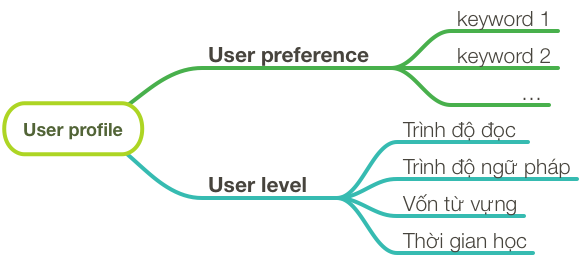
\includegraphics[scale=0.7]{userprofile}
    \else
      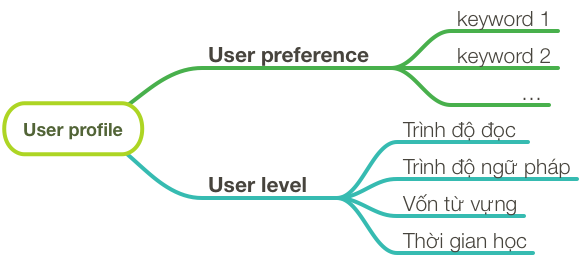
\includegraphics[scale=0.7]{userprofile}
    \fi
    \caption{User profile}
    \label{Userprofile}
  \end{center}
\end{figure}

\subsection{Xác định trình độ người dùng}

Để xác định trình độ Tiếng Anh của người dùng, tất cả các khía cạnh sau đây cần được khai thác:
\begin{itemize}
\item Thời điểm bắt đầu học
\item Trình độ đọc hiểu
\item Trình độ ngữ pháp
\item Vốn từ vựng
\end{itemize}

Bài kiểm tra tương tác CAT sẽ được sử dụng để đánh giá trình độ.Phương thức chọn câu hỏi và đánh giá bài thi CAT trong đề tài được xây dựng dựa trên mô hình Thử tỉ lệ xác suất nối tiếp \cite{welchfrick} (Sequential probability ratio test).\\ 

Nguyên lý căn bản nằm bên trong mô hình này là xác suất hợp lý rời rạc. Giả sử từ quan sát thực tế cho thấy thí sinh có trình độ tiếng Anh xuất sắc đạt trung bình 85/100 điểm trong bài thi, trong khi thí sinh có trình độ thấp chỉ đạt 35/100 điểm. Dưới góc nhìn hệ thống có thể coi nó như tập luật $if....else$ sau đây:

\begin{enumerate}
	\item Thí sinh có trình độ xuất sắc, đã nắm vững kiến thức và hiểu rõ câu hỏi cũng như phương pháp giải quyết, do vậy khả năng mà họ trả lời đúng câu hỏi sẽ là 85 \%. 
		\subitem Prob(Correct|Master) = .85 ($P_m$)
		\subitem Prob(Incorrect|Master) = .15
	\item Ngược lại, thí sinh có trình độ thấp, trả lời phần lớn dựa trên may rủi, giác quan thứ 6 của bản thân, do vậy khả năng mà họ trả lời đúng câu hỏi sẽ là 35 \%. 
		\subitem Prob(Correct|Nonmaster) = .35 ($P_n$)
		\subitem Prob(Incorrect|Nonmaster) = .75
\end{enumerate}  

Trong bài kiểm tra CAT, với câu hỏi bất kì phù hợp trình độ được chọn ra trong tập câu hỏi đưa cho thí sinh. Quan sát trả lời của thí sinh, xác suất khả năng trình độ sẽ được tính bằng:

\begin{equation}
PR = \dfrac{P_m^s(1-P_m)^f}{P_m^s(1-P_m)^f}
\end{equation}
trong đó $P_m = $ khả năng thí sinh trình độ xuất sắc trả lời đúng câu hỏi

$P_n = $ khả năng thí sinh trình độ thấp trả lời đúng câu hỏi

$s = $ tổng số câu hỏi thí sinh trả lời đúng 

$f = $ tổng số câu hỏi thí sinh trả lời sai 

Giá trị $PR$ sau đó sẽ được đem so sánh với tập luật:
\begin{itemize}
	\item Nếu $PR > UBN$ (Upper Bound Nonmastery: giá trị ngưỡng trên của độ không thuần thục) -> trình độ người dùng thấp hơn câu hỏi hiện tại, chọn câu hỏi tiếp theo ở trình độ thấp hơn để tiếp tục đánh giá .
	\item Nếu $PR < LBM$ (Lower Bound Mastery: giá trị ngưỡng dưới của độ thuần thục) -> trình độ người dùng nằm trên câu hỏi hiện tại, chọn câu hỏi tiếp theo ở trình độ cao hơn để tiếp tục đánh giá. 
	\item Nếu $UBN < PR < LBM$, kết quả hiện tại chưa đủ để đánh giá trình độ người dùng, chọn câu hỏi tiếp theo ở cùng trình độ để tiếp tục đánh giá.  
\end{itemize}


Trình độ của thí sinh được xác định khi $PR$ lớn hơn giá trị $UBN$ hoặc nhỏ hơn giá trị $LBM$. Tuy nhiên, xét trong trường hợp thực tế có khả năng xảy ra việc số lượng câu hỏi thí sinh trả lời sai bằng với số lượng câu hỏi thí sinh trả lời đúng. Điều này dẫn đến tình trạng thí sinh trả lời một số lượng lớn câu hỏi nhưng vẫn không xác định được trình độ. Điều kiện dừng sẽ được đưa vào để giải quyết trường hợp đó.

Hệ thống sẽ dừng bài kiểm tra đánh giá nếu như:
\begin{itemize}
	\item Nếu $PR > UBN$ và \textit{"độ khó hiện tại là thấp nhất"}
	\item Nếu $PR < LBM$ \textit{"độ khó hiện tại là cao nhất"}
	\item Nếu $UBN < PR < LBM$, số lượng câu hỏi hiện tại vượt \textit{ngưỡng câu hỏi}
\end{itemize}

Sau dây là mô hình đánh giá trình độ người dùng sử dụng trong đề tài:

\begin{figure}[H]
  \begin{center}
    %\leavevmode
    \ifpdf
      \includegraphics[scale=0.8]{cat}
    \else
      \includegraphics[scale=0.8]{cat}
    \fi
    \caption{Mô hình bài kiểm tra tương tác}
    \label{CATModel}
  \end{center}
\end{figure}

Trước tiên, trình độ ban đầu của người dùng sẽ được xác định qua câu hỏi "Bạn đã học tiếng Anh được bao lâu rồi". Trình độ của một người nào đó thường tỉ lệ thuận với thời gian họ bỏ ra để học.  do vậy ta có thể phần nào phán đoán được thông qua thông tin thời gian học. Đây là bước tiền đề trước khi đi vào thực hiện bài thi.

Tập câu hỏi đánh giá trình độ ban đầu, gồm hơn 70 câu hỏi lấy từ trang $EnglishJet$. Chúng được phân loại vào từng tập câu hỏi khác nhau theo các \textit{chủ đề}\{\textit{đọc hiểu, từ vựng, ngữ pháp}\} và \textit{trình độ}\{\textit{nhập môn, cơ bản, trung bình, khá, cao cấp}\}. Dựa trên trình độ hiện tại của người dùng, hệ thống sẽ chọn bất kì một câu hỏi trong tập câu hỏi cùng trình độ ra để kiểm tra. Sau khi kết thúc một chủ đề, trình độ hiện tại của người dùng sẽ được sử dụng làm trình độ ban đầu trong đánh giá chủ đề tiếp theo.

 Việc đánh giá kết quả được thực hiện theo tập luật đã đề cập ở phía trên. Dựa vào quan sát thử nghiệm trong thực tế, hệ thống đề xuất trong đề tài sử dụng các giá trị $UBN = 0.02$, $LBM = 7$ và \textit{ngưỡng câu hỏi} $= 5$.
 
 \subsection{Xác định nguyện vọng người dùng}
\section{Xây dựng mạng từ khoá}


